\chapter{Histogram View}
\label{sec:histo_view}

A Histogram View displays the distribution of one numerical variable as a histogram, approximating the statistical distribution of said varable. When started, it presents itself in the following manner.

\begin{figure}[H]
    \hspace*{-2cm}
    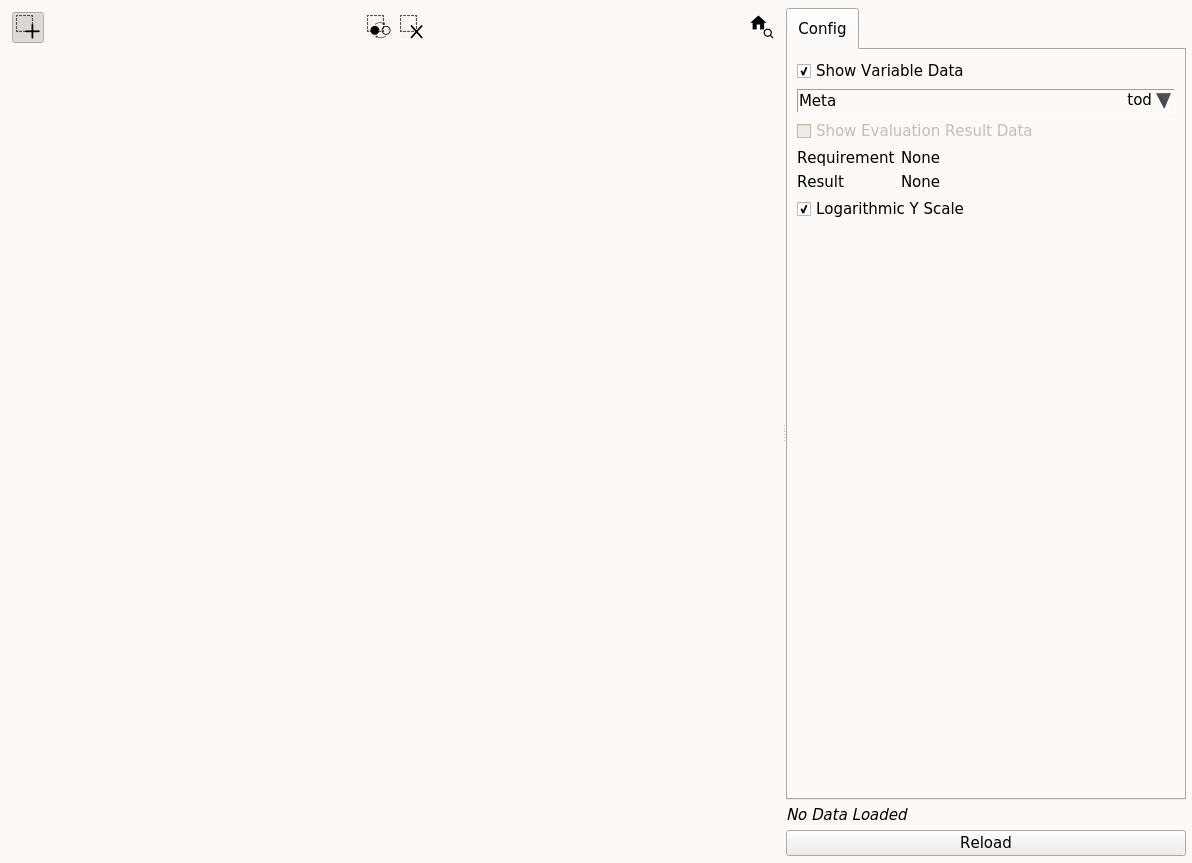
\includegraphics[width=18cm,frame]{figures/histogram_start.png}
  \caption{Histogram View startup}
\end{figure}

\section{Layout}

At the top, a (minimal) tool bar is shown, showing the currently selected tool and the available actions. \\

On the left side, the histogram is shown (if data has been loaded). \\

On the right side, a configuration area exists which allows configuration of what data is loaded and how it is displayed. \\

Both areas can be resized and hidden if wanted.

\section{Data Loading}

To load the data the mechanism described in Section \nameref{sec:load} or the 'Reload' button can be used. To filter the dataset, the mechanism described in Section \nameref{sec:filtering} can be used. \\

\begin{figure}[H]
    \hspace*{-2cm}
    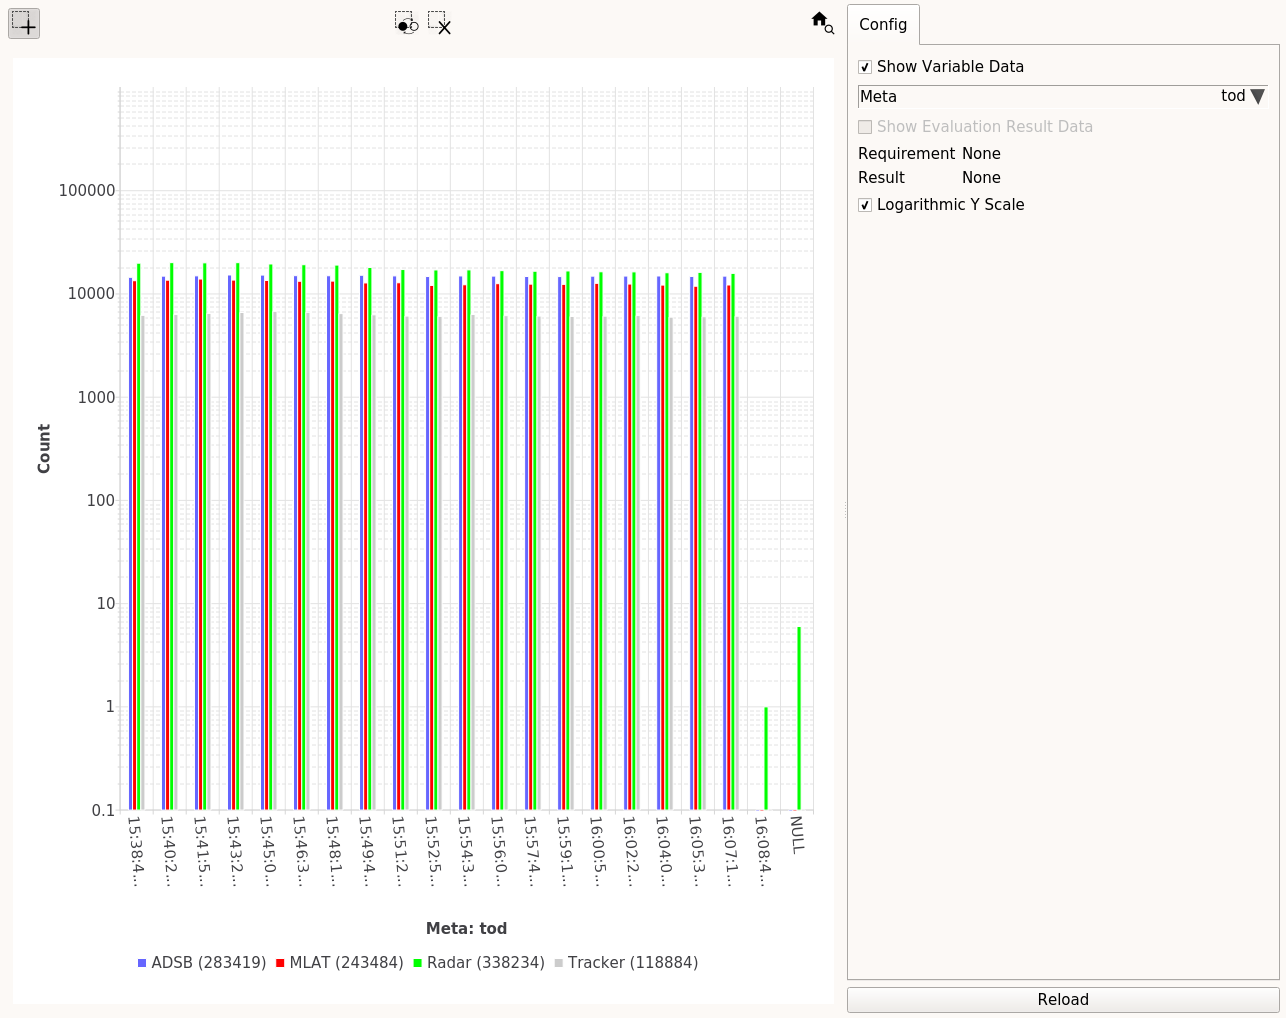
\includegraphics[width=18cm,frame]{figures/histogram_loaded.png}
  \caption{Histogram View after loading}
\end{figure}

On the x-axis the selected variable data is shown, in 20 bins (plus one optional NULL value bin), scaled between the minimum and maximum of the loaded data. On the y-axis the bin size per DBObject is shown (plus one optional for selected data), either in linear or logarithmic scale. \\


On the bottom a legend is shown giving the total counts of all data points. \\

In the current example the meta-variable 'tod' is used, showing the overall data rate per DBObject.


\section{Usage}

\subsection{Toolbar}

The first symbols switch between the mouse action modes, currently only one is available.

\begin{table}[H]
  \center
  \begin{tabular}{ | l | l | l |}
    \hline
    \textbf{Icon} & \textbf{Text} &  \textbf{Description} \\ \hline
    
\includegraphics[width=0.5cm,frame]{../../data/icons/select_action.png} & Select & Allows data selection \& de-selection \\ \hline
  \end{tabular}
  \caption{Toolbar mouse action modes}
\end{table}

The others provide general operations (shortcut refers to keyboard shortcut):

\begin{table}[H]
  \center
  \begin{tabular}{ | l | l | l | l |}
    \hline
    \textbf{Icon} & \textbf{Shortcut} &\textbf{Text} &  \textbf{Description} \\ \hline
    \includegraphics[width=0.5cm,frame]{../../data/icons/select_invert.png} & & Invert Selection & Selects all de-selected \& vice versa \\ \hline
    \includegraphics[width=0.5cm,frame]{../../data/icons/select_delete.png} & & Delete Selection & De-selects all target reports \\ \hline
    \includegraphics[width=0.5cm,frame]{../../data/icons/zoom_home.png} & & Zoom to Home & Pans/zooms to show all existing data \\ \hline
  \end{tabular}
  \caption{Toolbar operations}
\end{table} 

\subsection{Config Tab}

The top elements show which data variable is shown, which can either be a (selectable, numerical) variable or evaluation result data (if triggered from showing an evaluation result). In the first case, any numerical variable can be selected, which might require a reload operation. In the second case, the 'Requirement' and 'Result' fields indicate what evuluation result is presented. \\

The 'Logarithmic Y Scale' checkbox selects linear or logarithmic scale of the y-axis. \\

The 'Reload' button can be used to trigger a reload.

\subsection{Histogram}

\subsubsection{Zoom}

The mouse wheel can be used to zoom in or out of the presented data. This is in the current presentation only useful in limited circumstances. The space key can be used to reset to the default zoom (euqivalent to \includegraphics[width=0.5cm,frame]{../../data/icons/zoom_home.png}).

\subsubsection{Select Action}

Using the default action data can be selected. The first left mouse-button click starts selection (showing a red rectangle), the second click finalizes the selection. All data in all intersected bins is selected.

\begin{figure}[H]
    \hspace*{-2cm}
    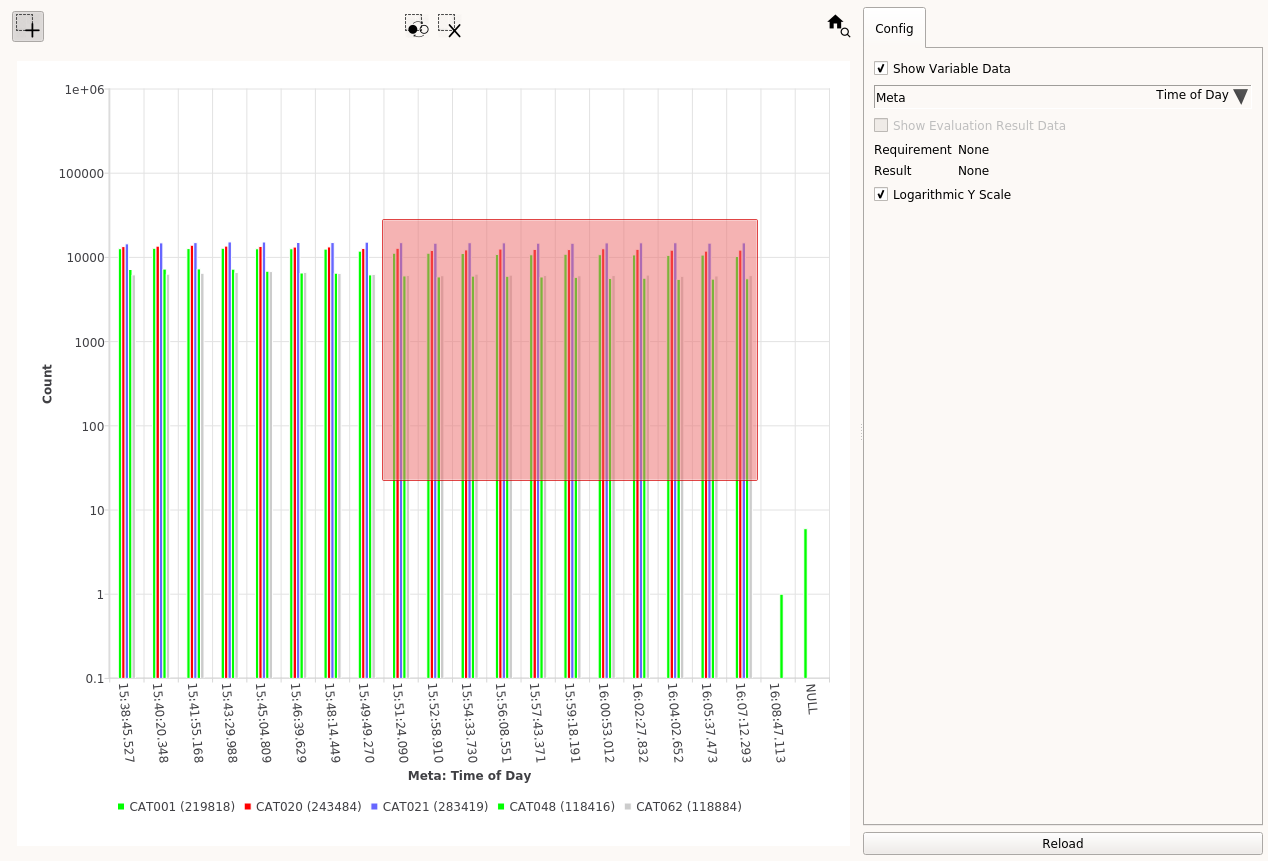
\includegraphics[width=18cm,frame]{figures/histogram_select.png}
  \caption{Histogram View data selection}
\end{figure}

The selected data is then presented in an extra 'Selected' column, grouping the count of all DBOObjects.

\begin{figure}[H]
    \hspace*{-2cm}
    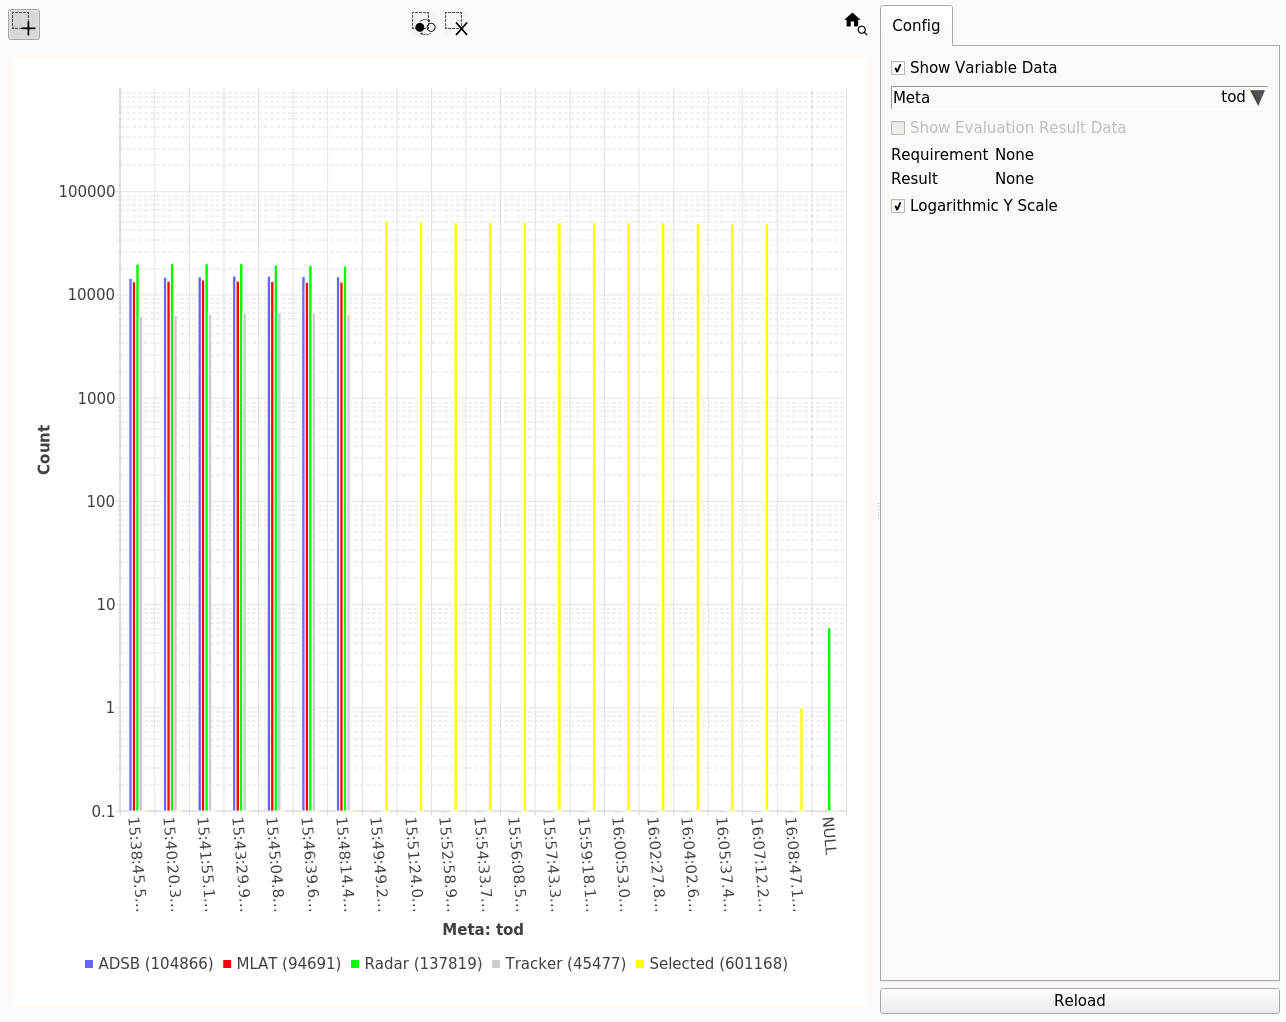
\includegraphics[width=18cm,frame]{figures/histogram_selected.png}
  \caption{Histogram View data selected}
\end{figure}

This allows selection of parts of the data based on the presented variable, allowing deeper analysis e.g. of dubious data. \\

The 'Invert Selection' \includegraphics[width=0.5cm,frame]{../../data/icons/select_invert.png} or 'Delete Selection' \includegraphics[width=0.5cm,frame]{../../data/icons/select_delete.png} actions allow for easier selection of the wanted target reports. \\

Also, if the 'Control' key is pressed during the second click, the new selected data is added to the already existing collection.

\subsection{Evaluation Result}

If, using the Evaluation feature a requirement result is presented, the respective data is shown in the histogram.

\begin{figure}[H]
    \hspace*{-2cm}
    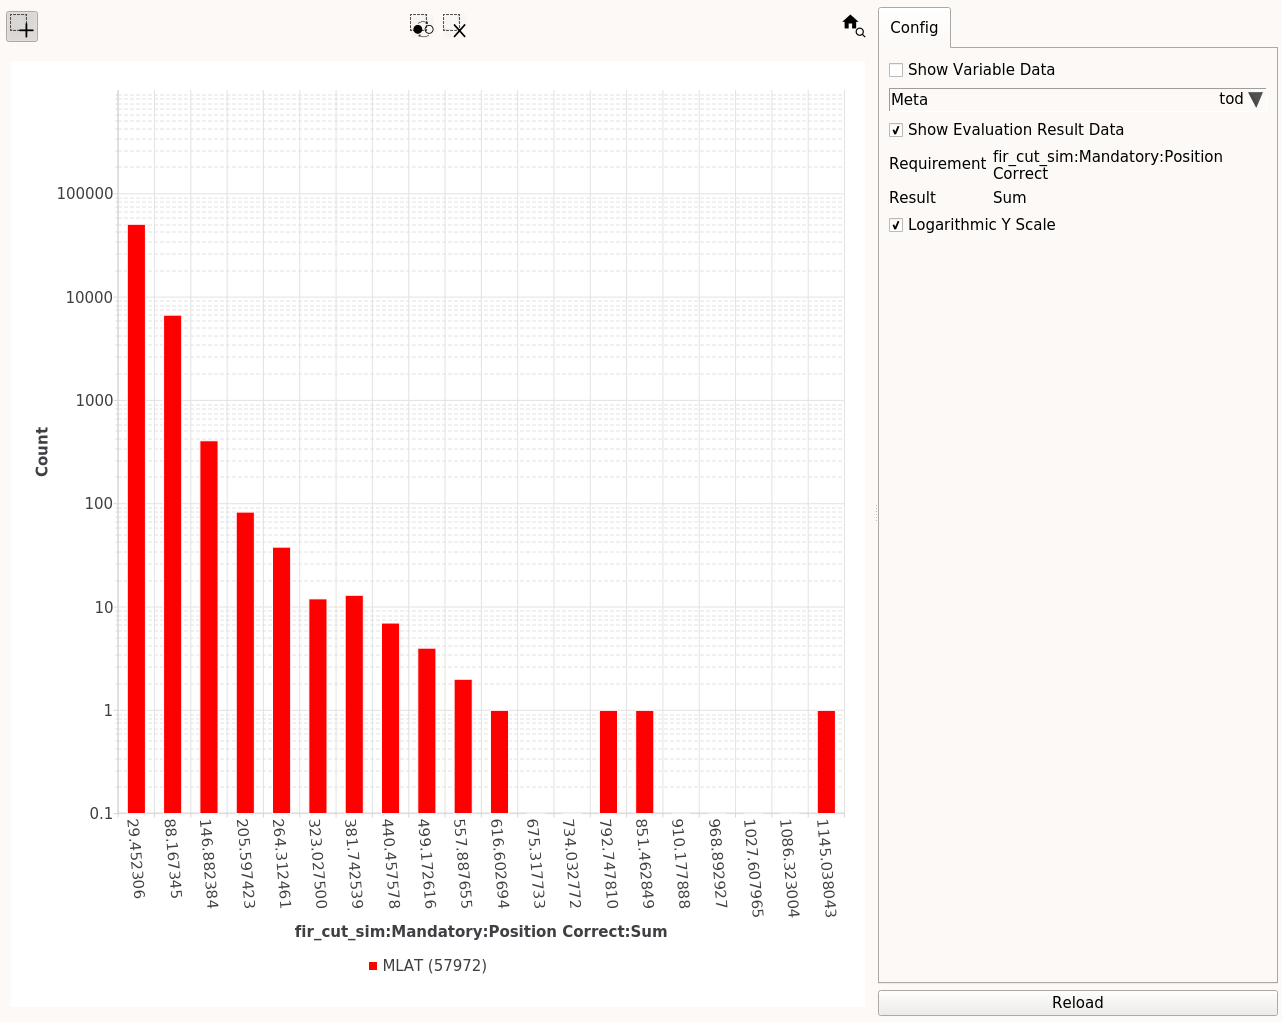
\includegraphics[width=18cm,frame]{figures/histogram_eval_pos_correct.png}
  \caption{Histogram View evaluation position correction result}
\end{figure}


\begin{figure}[H]
    \hspace*{-2cm}
    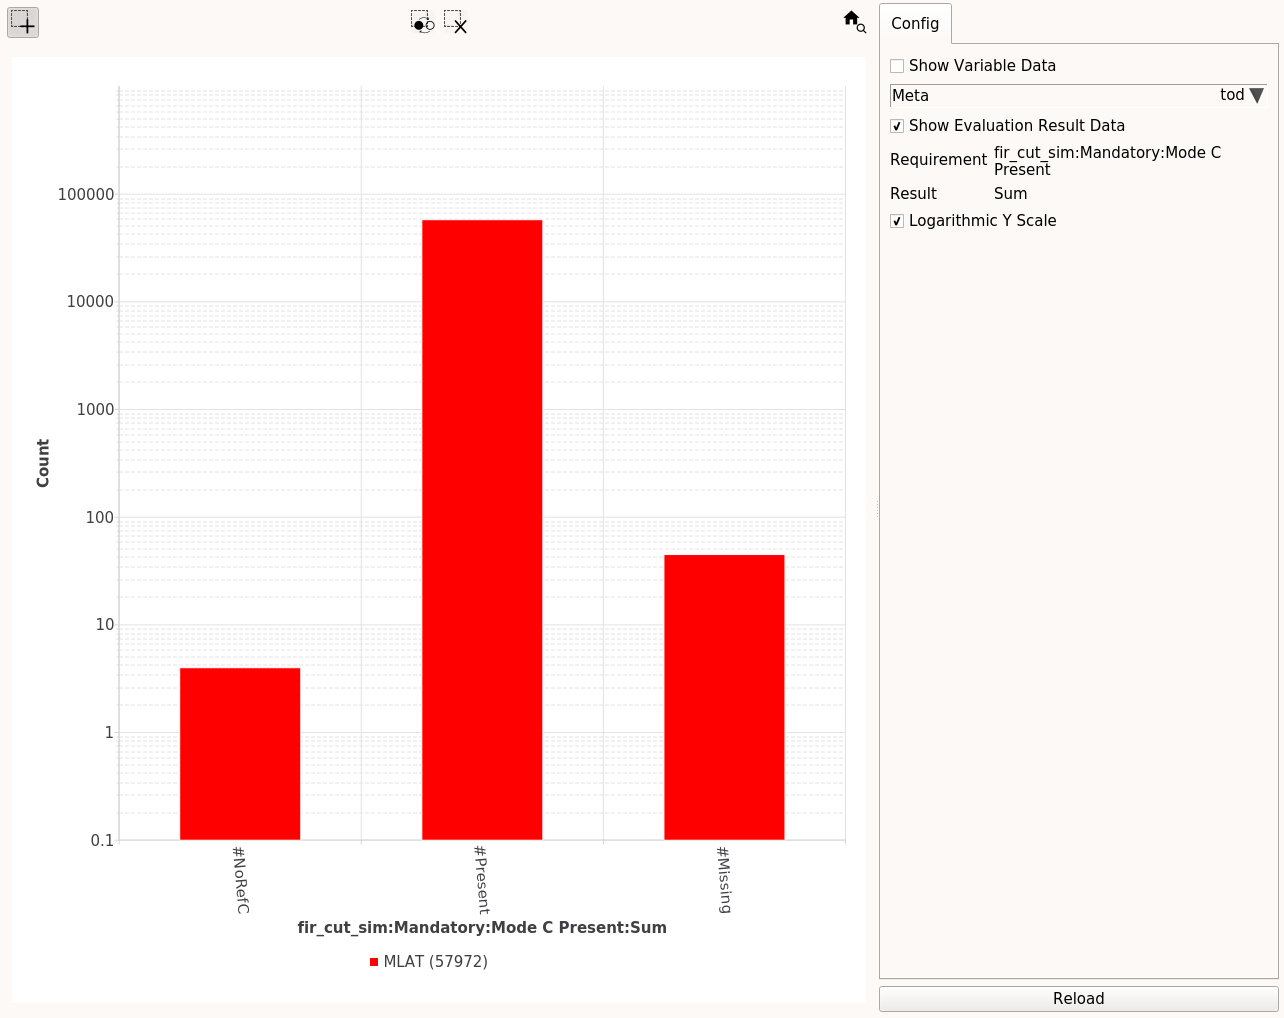
\includegraphics[width=18cm,frame]{figures/histogram_eval_mc.png}
  \caption{Histogram View Mode C present result}
\end{figure}

Please note that currently evalution result data can not be selected. This will be improved in one of the next versions.

